\documentclass[11pt,letterpaper,logo]{seu-paisys}

\usepackage[utf8]{inputenc}
\usepackage[T1]{fontenc}
\usepackage{hyperref}
\usepackage{url}
\usepackage{booktabs}
\usepackage{amsfonts}
\usepackage{nicefrac}
\usepackage{microtype}
\usepackage{xcolor}
\usepackage{graphicx}

\usepackage{multirow}
\usepackage{amsmath}
\usepackage{tabularx}
\usepackage{array}
\usepackage{CJKutf8}
\usepackage{xspace}

\newcommand{\system}{\texttt{Embodied.cpp}\xspace}
\usepackage{tikz}
\usetikzlibrary{arrows.meta}

\newcommand{\llamacpp}{llama.cpp}
\newcommand{\vlacpp}{vla.cpp}
\newcommand{\cmark}{\ding{51}}
\newcommand{\xmark}{\ding{55}}
\newcommand{\omark}{\ensuremath{\circ}}
\newcommand{\tmark}{\ensuremath{\triangle}}
\newcommand{\seumark}{
\includegraphics[height=1.2em]{logo-seu.pdf}}
\newcommand{\njumark}{
\includegraphics[height=1.2em]{logo-nju.jpg}}
\newcommand{\thumark}{
\includegraphics[height=1.2em]{logo-thu.pdf}}
\newcommand{\msmark}{
\includegraphics[height=1.2em]{logo-microsoft.pdf}}

\renewcommand{\today}{2026-07-01}
\setlength{\headheight}{66pt}

\title{\system: A Portable Inference Runtime of Embodied AI Models on Heterogeneous Robots}

\author{%
  {\large\textbf{Ling Xu}$^{1}$ \quad \textbf{Chuyu Han}$^{2}$ \quad \textbf{Borui Li}$^{1,\dagger}$ \quad \textbf{Hao Wu}$^{2,\dagger}$ \quad \textbf{Shiqi Jiang}$^{3}$ \quad \textbf{Ting Cao}$^{4}$ \quad \textbf{Chuanyou Li}$^{1}$ \quad \textbf{Sheng Zhong}$^{2}$ \quad \textbf{Shuai Wang}$^{1}$\\}
  \vspace{0.2em}
  {\normalsize 
  $^{1}$\ \seumark\ Southeast University \qquad 
  $^{2}$\ \njumark\ Nanjing University \qquad 
  $^{3}$\ \msmark\ Microsoft Research \qquad \qquad \qquad
  $^{4}$\ \thumark\ Institute for AI Industry Research (AIR), Tsinghua University }

  {\normalsize $^{\dagger}$Project Leader}
}

\begin{document}

%\begin{abstract}
%\end{abstract}

\begin{abstract}
\quad Embodied AI models now span vision-language-action (VLA) models and world-action models (WAMs), but practical deployment remains fragmented across model-specific Python stacks, backend assumptions, and robot-side glue code, especially on heterogeneous edge devices. Existing inference runtimes are designed mainly for request-response serving and therefore do not satisfy the runtime contract of embodied deployment: multi-rate execution inside closed-loop control, latency-first batch-1 inference on heterogeneous hardware, and extensible embodied interfaces beyond fixed token I/O. We present \textbf{\system}, a portable C++ inference runtime for embodied models. Based on an architectural analysis of representative VLA models and WAMs, \system captures a shared execution path and organizes it into five layers: input adapters, sequence builders, backbone execution, head plugins, and deployment adapters. The runtime provides modular multi-rate execution, latency-first fused inference, and extensible operator and I/O support, enabling deployment across heterogeneous devices, robots, and simulators through one backend abstraction. We evaluate \system on two VLA models, HY-VLA and pi0.5, and on a preliminary WAM benchmark using a LingBot-VA Transformer block. The VLA deployments achieve successful closed-loop execution with 100.0\% and 91.0\% task success rates, respectively. The WAM benchmark reduces block memory from 312.2 MiB to 88.1 MiB. These results show that \system improves deployment efficiency while preserving high accuracy across diverse embodied model architectures.

\quad Project Link: \href{https://github.com/SEU-PAISys/Embodied.cpp}{https://github.com/SEU-PAISys/Embodied.cpp}
\end{abstract}

\maketitle

%\section{Introduction}
%
%Embodied AI is advancing quickly, and its practical usage is increasingly shaped by a diverse set of model paradigms. Recent progress now spans vision-language-action (VLA) models and world-action models (WAMs). At the same time, the surrounding ecosystem for data, training, and simulation has become substantially stronger, supported by projects such as LeRobot, OpenVLA, Open X-Embodiment, ManiSkill, LIBERO, and Isaac Sim~\cite{lerobot,openvla,openx,maniskill,libero,isaacsim}. The central question is therefore no longer whether embodied models can be trained, but how an evolving family of such models can be turned into reliable robot-side systems.

\section{Introduction}

Academia and industry have already produced a rapidly growing set of embodied models. Recent systems now span vision-language-action (VLA) models and world-action models (WAMs), showing substantial progress in model architecture and capability~\cite{openvla,pi0,pi05,grootn1,lingbotva,wam-survey,li2026stop}. At the same time, the surrounding ecosystem for data, training, and simulation has also improved substantially through projects such as LeRobot, Open X-Embodiment, ManiSkill, LIBERO, and Isaac Sim~\cite{lerobot,openx,maniskill,libero,isaacsim}. But practical impact does not end at model construction. To become reliable robot-side systems, these models must run on heterogeneous and resource-constrained devices, from Jetson and RK-based boards to x86 edge boxes and workstation-class robots, without rebuilding the software stack for each new model family.

%That question is fundamentally a deployment question. Unlike cloud-oriented language or vision-language serving, embodied inference lives inside a control loop: observations arrive continuously, actions must be produced under timing constraints, and failures are expressed in physical behavior rather than degraded user experience. For robots, efficient on-device deployment is especially important. Robots keep moving while sensing and acting, and many tasks require high-precision, low-latency action generation. In practice, this means embodied models need to run locally on Jetson devices, RK-based boards, x86 edge boxes, or workstation-class robots with predictable latency and a manageable software stack.

Achieving this requires a unified inference runtime. Existing inference runtimes, however, do not yet provide such support. General LLM or VLM runtimes are designed for request-response serving, relatively uniform token interfaces, and throughput-oriented optimization~\cite{llama-cpp,onnxruntime,sglang,vllm-omni}. Embodied inference, by contrast, lives inside a closed-loop interaction process with robot- and simulator-side dependencies. As a result, even a strong checkpoint still has to be stitched into Python research code, backend-specific inference paths, handwritten sensor wrappers, and platform-specific control logic before it can act on a robot. As embodied architectures diversify, this integration burden only grows, making a portable inference runtime for embodied AI models increasingly necessary.

%Current deployment practice does not yet meet that need. Even when a strong checkpoint is available, real deployment is still fragmented across Python-heavy research code, backend-specific inference paths, hand-written sensor wrappers, and platform-specific control loops. This makes embodied deployment a recurring integration effort rather than a reusable systems layer. The problem becomes even sharper as paradigms diversify: each new model family seems to arrive with a slightly different execution story, encouraging teams to rebuild the same infrastructure again and again.

The challenge arises because embodied deployment fundamentally changes the runtime contract. Compared with conventional LLM or VLM serving, an embodied inference runtime must satisfy three key requirements. \textbf{(1) Multi-rate execution.} Embodied inference is not a single synchronous forward pass: perception encoders, transformer backbones, predictive branches, and action heads may need to run at different rates inside the same control loop, as increasingly visible in hierarchical and fast-slow VLA systems as well as recent WAMs~\cite{pi05,grootn1,lingbotva}. \textbf{(2) Latency-first closed-loop control.} The optimization target is not throughput but stable closed-loop control, which requires low latency, low jitter, and efficient batch-1 execution on heterogeneous edge hardware. \textbf{(3) Extensible embodied interfaces.} Embodied deployment must go beyond fixed token I/O and absorb custom operators, embodied multimodal inputs, and heterogeneous outputs ranging from action chunks to predicted futures. These are not peripheral engineering details; together they define the runtime contract that a practical embodied inference runtime must satisfy.

%This report argues that the right response is a dedicated runtime substrate for embodied deployment. We position \system as a portable C++ runtime that provides a unified execution layer for embodied models across heterogeneous edge devices and robots. The choice of C++ and portability is therefore a systems decision, not a branding choice: a portable C++ runtime offers a small dependency surface, direct control over memory and scheduling, predictable latency, and a practical path to deployment across different robot-side devices. Our core claim is that, despite rapid model evolution, recent embodied systems already expose enough architectural regularity to support such a stable runtime abstraction.

Motivated by these observations, we present \system, a portable C++ inference runtime for embodied models. Its design directly addresses the three challenges: modular multi-rate execution decouples components with different refresh frequencies; latency-first fused execution targets predictable small-batch control on heterogeneous devices; and extensible operator and embodied I/O support turns model-specific heads, interfaces, and backends into pluggable runtime modules instead of one-off glue code. These principles are realized in a unified five-layer architecture spanning input adapters, sequence builders, backbone execution, head plugins, and deployment adapters. The result is an inference runtime with a stable reusable core, while still leaving enough extension surface for new embodied model variants.

% The core bet is that, despite rapid model evolution, recent embodied systems already expose enough architectural regularity to support a stable runtime abstraction. We make that case with the architecture in Section~2 and the VLA deployment results in Section~3.


We make three contributions:
\begin{itemize}
    \item An architectural analysis of representative embodied models spanning vision-language-action (VLA) models and world-action models (WAMs), revealing a shared execution path whose main divergences are confined to a small set of pluggable heads and predictive modules.
    \item The design of \system as a portable C++ inference runtime that maps this shared path into five layers: input adapters, sequence builders, backbone execution, head plugins, and deployment adapters, with backend abstraction for heterogeneous edge devices.
    \item We evaluate \system on two widely used VLA models and one representative WAM benchmark, showing improved efficiency while maintaining high accuracy.
\end{itemize}

\section{Related Work and Motivation}

\subsection{Embodied AI Model and Architectural Analysis}

From an inference-runtime perspective, recent embodied models can be organized into two online families: vision-language-action (VLA) models and world-action models (WAMs). As summarized in Figure~\ref{fig:architecture-taxonomy} and Table~\ref{tab:architecture-serving}, VLA models primarily realize a perception-to-action path, while WAMs make future prediction an explicit part of online control~\cite{openvla,pi0,wam-survey}. This split matters directly to systems design because it determines whether the runtime mainly executes an action policy or must jointly maintain predictive state and action generation.

Within the VLA family, the architectural progression is from monolithic action generation to increasingly structured modular execution. AR-Token VLA models such as RT-2 and OpenVLA use one shared backbone to autoregressively generate action tokens~\cite{rt2,openvla}. VLM-Backboned VLA models such as Octo, pi0, pi0.5, and MuseVLA still rely on a strong shared visual-language backbone, but pair it with more explicit continuous-action heads~\cite{octo,pi0,pi05,musevla}. More recent systems then branch into two modular directions. Hierarchical VLA models split semantic planning from low-level control, with a planner producing subgoals for a downstream controller, as in Hi Robot, GeneralVLA, RT-H, and Gemini Robotics 1.5~\cite{hirobot,generalvla,rth,geminirobotics15}. Asynchronous VLA models instead split execution by time scale: decoupled modules run at different rates and coordinate through buffered state, as in GR00T N1, Fast-in-Slow, and DAM-VLA~\cite{grootn1,fis,damvla}. The key runtime takeaway is that even within VLA models, the execution unit is no longer uniformly a single synchronous forward pass.

\begin{figure*}[t]
\centering
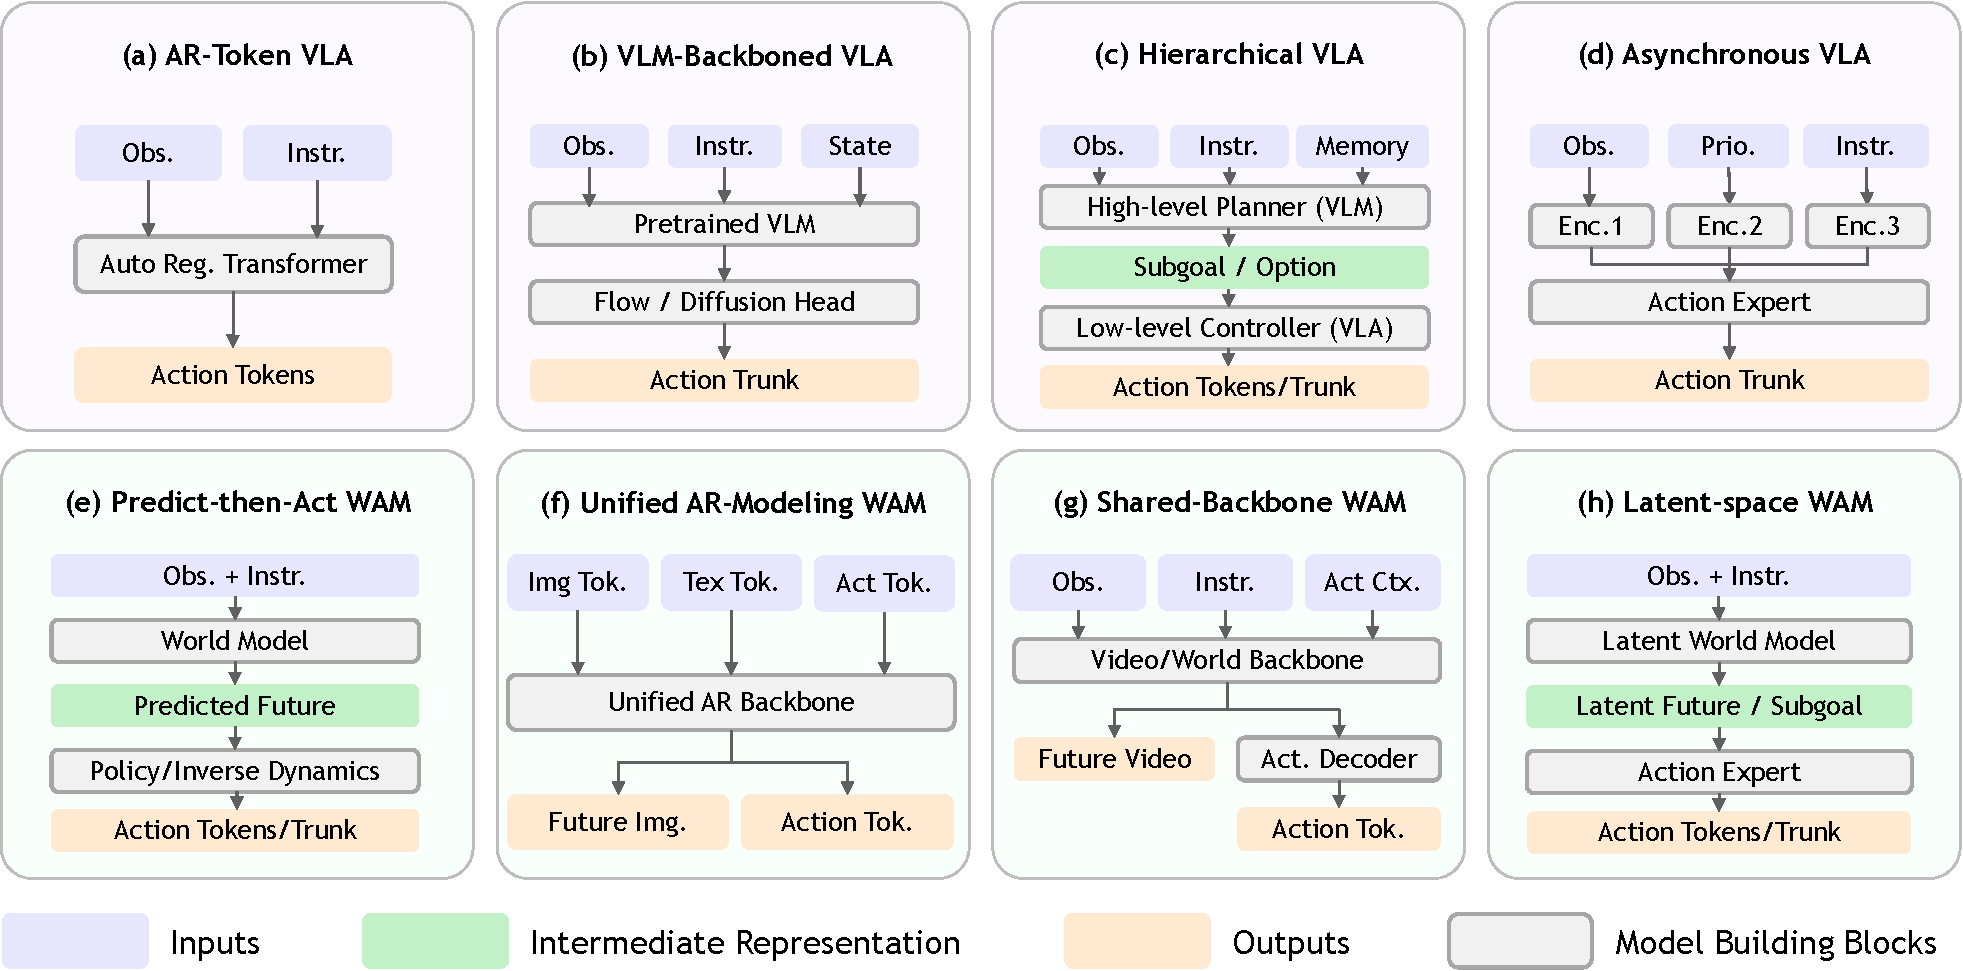
\includegraphics[width=\textwidth]{model-comparison.pdf}
\caption{Architectural taxonomy of embodied models. We first separate VLA models (a-d) from WAMs (e-h), and then organize each family by internal inference structure.}
\label{fig:architecture-taxonomy}
\end{figure*}

The WAM family is organized by how future prediction is coupled with action generation. Predict-then-Act WAMs such as UniPi keep the two stages explicit: a world model predicts future states, and a downstream action expert consumes them~\cite{unipi}. Unified AR-Modeling WAMs collapse future modeling and action generation into one autoregressive token space, as in WorldVLA and LingBot-VA~\cite{worldvla,lingbotva}. Shared-Backbone WAMs reuse one backbone across world modeling and action generation, while still exposing separate blocks that can potentially be scheduled or extended independently, as in DreamZero, Fast-WAM, Cosmos Policy, and the Unified Video Action Model (UWM)~\cite{dreamzero,fastwam,cosmospolicy,uwm}. Latent-space WAMs compress the predictive path further by generating a compact latent future or subgoal for a downstream action expert, as in LaWAM and Being-H0.7~\cite{lawam,beingh07}. Compared with VLA models, WAMs therefore broaden the runtime contract from direct action decoding to coordinated management of predictive computation and control computation.

\begin{table*}[t]
\centering
\caption{Architecture-oriented comparison of embodied AI models.}
\label{tab:architecture-serving}
\footnotesize
\setlength{\tabcolsep}{3.8pt}
\renewcommand{\arraystretch}{1.14}
\begin{tabularx}{\textwidth}{>{\raggedright\arraybackslash}p{0.22\textwidth} >{\raggedright\arraybackslash}p{0.31\textwidth} >{\centering\arraybackslash}p{0.09\textwidth} X}
\toprule
\rowcolor{black!5}
\textbf{Subtype} & \textbf{Architectural Characteristic} & \textbf{Structure} & \textbf{Representative Models} \\
\midrule
\rowcolor{black!2}
\multicolumn{4}{l}{\textbf{Vision-Language-Action (VLA) Models}} \\
AR-Token VLA & One backbone autoregressively generates action tokens. & Monolithic & OpenVLA~\cite{openvla}, RT-2~\cite{rt2} \\
VLM-Backboned VLA & A shared pretrained VLM feeds a continuous action head. & Modular & Octo~\cite{octo}, pi0~\cite{pi0}, pi0.5~\cite{pi05}, MuseVLA~\cite{musevla} \\
Hierarchical VLA & A high-level planner produces subgoals for a low-level controller. & Modular & Hi Robot~\cite{hirobot}, GeneralVLA~\cite{generalvla}, RT-H~\cite{rth}, Gemini Robotics 1.5~\cite{geminirobotics15} \\
Asynchronous VLA & Decoupled modules run at different rates through buffered coordination. & Modular & GR00T N1~\cite{grootn1}, Fast-in-Slow~\cite{fis}, DAM-VLA~\cite{damvla} \\
\addlinespace[2pt]
\rowcolor{black!2}
\multicolumn{4}{l}{\textbf{World-Action Models (WAM)}} \\
Predict-then-Act WAM & An explicit world model predicts future states before a downstream action expert acts. & Modular & UniPi~\cite{unipi} \\
Unified AR-Modeling WAM & Future world and robotic action are jointly generated in one autoregressive token space. & Monolithic & WorldVLA~\cite{worldvla}, LingBot-VA~\cite{lingbotva} \\
Shared-Backbone WAM & World modeling and action generation share one backbone, while auxiliary blocks can run at different rates. & Modular & DreamZero~\cite{dreamzero}, Fast-WAM~\cite{fastwam}, Cosmos Policy~\cite{cosmospolicy}, UWM~\cite{uwm} \\
Latent-space WAM & A compact latent future or subgoal is predicted and then consumed by an action expert. & Modular & LaWAM~\cite{lawam}, Being-H0.7~\cite{beingh07} \\
\bottomrule
\end{tabularx}
\end{table*}

Taken together, Figure~\ref{fig:architecture-taxonomy} and Table~\ref{tab:architecture-serving} suggest three implications for inference runtime design. First, structural organization is now a first-class model property: some systems remain monolithic, but many recent ones are better understood as interacting planner, backbone, world-model, and action modules. Second, intermediate states such as subgoals, buffered context, predicted futures, and latent futures have become explicit runtime objects rather than hidden internal details. Third, timing structure is increasingly model-defined, especially in hierarchical and asynchronous systems, so a practical embodied inference runtime must support stateful multi-component orchestration instead of assuming one uniform synchronous request-response path.

\subsection{Existing Inference Runtimes for AI Models}

AI model inference is well-studied in the past few years~\cite{wu2021pecam,wu2020emo,zeng2025h2o,li2024agent,li2025infscaler,li2025mobilora}.
General-purpose inference runtimes already cover much of the shared execution substrate. \llamacpp{} emphasizes lightweight C/C++ local inference, broad hardware coverage, and practical packaging~\cite{llama-cpp}; ONNX Runtime provides cross-platform acceleration through multiple execution providers~\cite{onnxruntime}; and serving systems such as SGLang and vLLM-Omni target large-scale LLM/VLM inference with richer multimodal pipelines~\cite{sglang,vllm-omni}. These systems are strong inference runtimes, but they primarily target request-response workloads with relatively uniform interfaces.

Embodied settings impose a different contract: closed-loop control, heterogeneous inputs and outputs, persistent state, batch-1 latency sensitivity, and direct robot or simulator integration. Simulation platforms such as ManiSkill, LIBERO, and Isaac Sim are important for training and benchmarking~\cite{maniskill,libero,isaacsim}, but they are not themselves embodied inference runtimes. The closest recent step is \vlacpp{}, which brings seven VLA architectures into one portable C++ inference runtime and reports execution from consumer GPUs to embedded devices together with an on-robot stress test~\cite{vla-cpp}. This is an important milestone, but it remains VLA-centric.

Table~\ref{tab:runtime-compare} makes the gap concrete from two complementary angles: model-family coverage and deployment-facing capability. The first question is whether a runtime directly supports VLA models or WAMs, and whether it provides explicit optimization support for modular multi-component models rather than only monolithic inference graphs. The second is whether it can actually carry those models to embodied deployment, including edge execution, heterogeneous-device cooperation, and direct connection to robots or simulators. Existing systems are either generic inference runtimes without first-class embodied model support, or embodied inference runtimes specialized to only one model family.

\begin{table*}[t]
\centering
\caption{Comparison of inference runtimes from the perspective of embodied model coverage and deployment readiness. `VLA' and `WAM' denote first-class support for the corresponding embodied model families. `Modular' denotes support or optimization for multi-component embodied models rather than only monolithic inference graphs. `Edge' denotes whether the runtime can run with deployment-oriented optimization on edge or end-side devices. `Hetero. HW' denotes whether one runtime can jointly use heterogeneous devices rather than only switch among backends. \cmark: native support. \xmark: unsupported. \omark: achievable only with substantial custom integration. \tmark: limited or partial support.}
\label{tab:runtime-compare}
\footnotesize
\setlength{\tabcolsep}{4.1pt}
\renewcommand{\arraystretch}{1.14}
\begin{tabularx}{\textwidth}{>{\raggedright\arraybackslash}X >{\centering\arraybackslash}p{0.07\textwidth} >{\centering\arraybackslash}p{0.07\textwidth} >{\centering\arraybackslash}p{0.09\textwidth} >{\centering\arraybackslash}p{0.07\textwidth} >{\centering\arraybackslash}p{0.11\textwidth} >{\centering\arraybackslash}p{0.08\textwidth} >{\centering\arraybackslash}p{0.10\textwidth}}
\toprule
\rowcolor{black!5}
\textbf{System} & \textbf{VLA} & \textbf{WAM} & \textbf{Modular} & \textbf{Edge} & \textbf{Hetero. HW} & \textbf{Robot} & \textbf{Simulator} \\
\midrule
\llamacpp{}~\cite{llama-cpp} & \xmark & \xmark & \xmark & \cmark & \tmark & \xmark & \xmark \\
\mbox{ONNX Runtime}~\cite{onnxruntime} & \omark & \omark & \omark & \cmark & \cmark & \xmark & \xmark \\
\textsc{SGLang}~\cite{sglang} & \xmark & \xmark & \xmark & \xmark & \xmark & \xmark & \xmark \\
\textsc{vLLM-Omni}~\cite{vllm-omni} & \omark & \omark & \tmark & \xmark & \tmark & \xmark & \xmark \\
\vlacpp{}~\cite{vla-cpp} & \cmark & \xmark & \tmark & \cmark & \tmark & \cmark & \tmark \\
\system{} (ours) & \cmark & \cmark & \cmark & \cmark & \cmark & \cmark & \cmark \\
\bottomrule
\end{tabularx}
\end{table*}

%The main gap is therefore not raw inference alone. What remains underbuilt is a deployment substrate that simultaneously supports multiple embodied paradigms, portable edge execution, embodied-aware packaging, and direct integration with robot-side control loops. \system is designed to occupy that systems layer.

Overall, existing systems still stop short of first-class embodied model coverage, modular-model optimization, and direct deployment interfaces. What remains underbuilt is an embodied inference runtime that jointly supports both VLA and WAM execution while also landing on edge devices, heterogeneous hardware, robots, and simulators.

\section{Project Overview}

\subsection{Challenges}

Embodied deployment should first be understood by contrast with traditional LLM and VLM inference. Conventional language or multimodal serving usually assumes a mostly synchronous request-response path, a relatively uniform token interface, and throughput-oriented optimization over large batches or many concurrent users. \system faces a different setting: embodied models run inside closed-loop control, combine multiple heterogeneous modules, and must remain deployable on robot-side hardware while absorbing new model families over time. For an open-source embodied inference runtime project, these differences collapse into three practical system challenges, each of which directly shapes the design of \system.

\begin{itemize}
    \item \textbf{1. Multi-rate execution.}
    As an open-source project, \system must support not only today's embodied models, but also the optimizations that future embodied architectures may require. This is difficult because many modern embodied systems are no longer monolithic. VLA models and WAMs are increasingly assembled from multiple modules, such as perception encoders, transformer backbones, predictive branches, and action heads. Unlike a conventional LLM runtime, efficient embodied inference does not always require every module to run at every step. A perception stack may refresh less frequently, a predictive branch may run only when future estimation is needed, and an action head may need to execute at a much higher control rate.

    \item \textbf{2. Latency-first closed-loop control.}
    Embodied deployment also raises a harder performance problem than ordinary cloud inference. In many robotics settings, execution is effectively batch-1: a single robot or simulator must receive actions continuously, with low latency, low jitter, and predictable timing behavior. At the same time, deployment targets are heterogeneous, spanning Jetson devices, RK-based platforms, x86 edge boxes, and workstation-class systems. This creates a tension between latency-first execution and the fused-inference techniques needed to make small-batch execution efficient across different backends and devices.

    \item \textbf{3. Extensible embodied interfaces.}
    Finally, implementing an embodied inference runtime is not only a scheduling problem. New model families regularly introduce new dependency stacks, larger custom operators, and new input/output conventions. A practical open-source inference runtime must therefore absorb model-specific libraries, cover a broader operator surface, and support new embodied data types on both sides of the interface. Inputs may include images, language, proprioception, history, force or tactile signals, and simulator-provided state. Outputs may be discrete action tokens, continuous action vectors, action chunks, world predictions, or intermediate control representations.
\end{itemize}

Taken together, these challenges explain why embodied deployment should not be framed as a small extension of an LLM runtime. The reusable substrate remains real and important, especially around multimodal projection, transformer-style execution, backend portability, and operator reuse. But the top-level contract has shifted from token serving to embodied control, and an open runtime must remain extensible enough to absorb future embodied optimizations rather than hard-coding today's model structure.

\subsection{Design Principles and Runtime Architecture}

These challenges, in turn, motivate three design principles of \system:
\begin{itemize}
    \item \textbf{1. Modular multi-rate execution.} \system should expose explicit execution units, pluggable modules, shared state or feature pools, and configurable refresh policies so that different components can run at different rates without forcing a single synchronous path.
    \item \textbf{2. Latency-first fused execution.} \system should prioritize stable control performance while still supporting graph replay, buffer reuse, operator fusion, backend-specific dispatch, and careful host-device data movement for efficient small-batch inference on heterogeneous devices.
    \item \textbf{3. Extensible operator and I/O support.} \system should provide typed embodied interfaces, pluggable heads, first-class deployment adapters, and enough backend and operator coverage to make new embodied paradigms implementable without rebuilding the surrounding runtime each time.
\end{itemize}

The model-side analysis in Section~2 and the runtime gap in Table~\ref{tab:runtime-compare} together motivate a runtime architecture that stays uniform at the deployment boundary while remaining extensible inside. Recent systems suggest three complementary lessons: \vlacpp{} shows that a broad family of VLA models can be organized around one shared inference path and one portable bundle format~\cite{vla-cpp}; Pie shows the value of separating a fixed execution substrate from a programmable control layer~\cite{pie}; and FlashRT shows that latency-first execution benefits from treating execution state as a first-class runtime object rather than as an implicit cache~\cite{flashrt}. \system combines these lessons in a form specialized for embodied deployment.

\begin{figure*}[t]
\centering

\includegraphics[width=\textwidth]{overview.pdf}
\caption{Project overview of \system. Diverse sensors and datasets enter through input adapters, model execution is unified around one embodied-model runtime that covers VLA models, WAMs, and future variants, and outputs are bridged to simulators and real robots through deployment adapters. Beneath this shared path, three runtime capabilities directly address the core challenges: modular multi-rate execution, latency-first batch-1 execution on heterogeneous hardware, and an embodied AI kernel warehouse for reusable operators and model-specific kernels.}
\label{fig:system-architecture}
\end{figure*}

Figure~\ref{fig:system-architecture} summarizes this design at a high level. On the left, \emph{input adapters} absorb both online sensor streams and offline dataset samples, so cameras, force or tactile signals, IMU data, and benchmark datasets enter the runtime through one typed embodied interface. In the center, \system maintains one shared embodied-model execution zone that can host VLA models, WAMs, and future embodied variants, while preserving explicit interfaces for future prediction, action experts, and final action generation. Beneath this model zone, three supporting subsystems directly mirror the challenges in Section~3.1: \emph{modular multi-rate execution} handles decoupled scheduling and runtime state, \emph{latency-first batch-1 execution on heterogeneous hardware} targets low-latency deployment across CPUs, GPUs, NPUs, and other accelerators, and the \emph{embodied AI kernel warehouse} collects reusable operators and model-specific kernels needed by evolving embodied architectures. On the right, \emph{output adapters} bridge runtime outputs to simulators and real-world robot software stacks. In this way, \system keeps the deployment boundary stable even as model structure, hardware targets, and embodied interfaces continue to evolve.

\section{Evaluation}

This revision reports two kinds of evidence: closed-loop results for two VLA models, HY-VLA and pi0.5, and a preliminary WAM microbenchmark on LingBot-VA. Full LingBot-VA closed-loop results are not included because the complete model is not yet stable on the constrained local edge setup used in this draft.

\noindent\textbf{VLA model evaluation.} We evaluate HY-VLA and pi0.5 through the C++ deployment path. HY-VLA is tested on the RoboTwin \texttt{place\_empty\_cup} task with its corresponding checkpoint, and pi0.5 is tested with its corresponding C++ deployment configuration. We report success rate, action chunk length, server-side inference latency, amortized environment-step latency, and peak GPU memory.


\begin{table}[t]
\centering
\caption{VLA deployment results.}
\label{tab:vla_deployment_results}
\footnotesize
\setlength{\tabcolsep}{2.8pt}
\renewcommand{\arraystretch}{1.14}
\begin{tabularx}{\columnwidth}{@{}>{\raggedright\arraybackslash}p{0.13\columnwidth} >{\raggedright\arraybackslash}p{0.17\columnwidth} >{\centering\arraybackslash}p{0.10\columnwidth} >{\centering\arraybackslash}X >{\centering\arraybackslash}p{0.09\columnwidth} >{\centering\arraybackslash}p{0.10\columnwidth} >{\centering\arraybackslash}p{0.13\columnwidth}@{}}
\toprule
\rowcolor{black!5}
\shortstack{\textbf{Deployed}\\\textbf{Model}} & \shortstack{\textbf{Model}\\\textbf{Backbone}} & \shortstack{\textbf{Action}\\\textbf{Chunk}} & \shortstack{\textbf{Success}\\\textbf{Rate (\%)}} & \shortstack{\textbf{Step}\\\textbf{(ms)}} & \shortstack{\textbf{Inf.}\\\textbf{(ms)}} & \shortstack{\textbf{VRAM}\\\textbf{(MiB)}} \\
\midrule
HY-VLA & Hunyuan-VL & 20 & \shortstack{100.0\\{[83.9, 100.0]}} & 735.9 & 1340.3 & 6850 \\
pi0.5 & PaliGemma & 50 & \shortstack{91.0\\{[86, 94]}} & 56.85 & 266.6 & 6546 \\
\bottomrule
\end{tabularx}
\end{table}

Table~\ref{tab:vla_deployment_results} shows that both models run correctly through the C++ runtime while preserving task behavior. HY-VLA reaches a 100.0\% success rate on the evaluated RoboTwin task. Its latency is higher than pi0.5 because it uses a larger Hunyuan-VL backbone, three-view inputs, and a video-history/MEM vision path. By contrast, pi0.5 uses a lighter PaliGemma backbone and a longer action chunk, which lowers the amortized step cost. Together, these results show that \system can support different VLA architectures within one C++ runtime, while latency and memory still depend on backbone size, visual input complexity, and action chunking.

\noindent\textbf{WAM evaluation.} For a preliminary WAM evaluation, we use LingBot-VA. Because the full model is not yet stable on the constrained local edge device, we benchmark only its first Transformer block and compare the original PyTorch implementation with the corresponding \system implementation.

\begin{table}[t]
\centering
\caption{LingBot-VA single-block quantization microbenchmark.}
\label{tab:lingbot_block_quant}
\scriptsize
\setlength{\tabcolsep}{2.0pt}
\renewcommand{\arraystretch}{1.14}
\begin{tabularx}{\columnwidth}{@{}>{\raggedright\arraybackslash}p{0.24\columnwidth} >{\centering\arraybackslash}p{0.13\columnwidth} >{\centering\arraybackslash}p{0.16\columnwidth} >{\centering\arraybackslash}p{0.16\columnwidth} >{\centering\arraybackslash}p{0.14\columnwidth} >{\centering\arraybackslash}X@{}}
\toprule
\rowcolor{black!5}
\shortstack{\textbf{Inference}\\\textbf{Runtime}} & \shortstack{\textbf{Model}\\\textbf{Quantization}} & \shortstack{\textbf{Latency}\\\textbf{/ block (ms)}} & \shortstack{\textbf{Memory}\\\textbf{/ block (MiB)}} & \shortstack{\textbf{MAE}\\$\downarrow$} & \shortstack{\textbf{Cosine}\\$\uparrow$} \\
\midrule
Python original & BF16 & 3.236 & 312.2 & $0$ & $1$ \\
\system & Q4\_K & 3.171 & 88.1 & $< 3.3 \times 10^{-2}$ & $> 9.997 \times 10^{-1}$ \\
\bottomrule
\end{tabularx}
\end{table}

Table~\ref{tab:lingbot_block_quant} reports the single-block results. The Python baseline uses the original \texttt{WanTransformerBlock} with BF16 weights, while the C++ path uses the corresponding GGUF Q4\_K quantized block. Latency is measured after warmup and includes only backend computation for one Transformer block, excluding request parsing, tensor staging, output post-processing, and other server-side overheads. Memory denotes resident weight memory for the measured block.

Using 100 random input samples, we compare the C++ Q4\_K block against the Python BF16 block with mean absolute error (MAE) and cosine similarity. The quantized C++ block reduces resident weight memory from 312.2 MiB to 88.1 MiB while keeping MAE below $3.3 \times 10^{-2}$ and cosine similarity above $9.997 \times 10^{-1}$. This is not a full WAM closed-loop result, but it provides initial evidence that \system can host and validate WAM-side Transformer components with large memory savings and very limited output drift.

%\section{Conclusion}
%
%Embodied models are becoming more diverse, but deployment infrastructure remains comparatively underdeveloped. \system addresses this gap by framing embodied deployment as a portable C++ runtime problem rather than as a collection of model-specific integration scripts. The resulting design emphasizes unified execution, backend portability, operator extensibility, and robot-side integration across heterogeneous edge devices and robots.
%
%As embodied paradigms continue to evolve, the need for a stable deployment substrate will only become more important. \system is intended to provide that substrate by making embodied models easier to run, compare, and integrate in practical edge and robot settings.





\section{Conclusion}

The evidence from recent models points in one direction: embodied deployment is converging on a shared execution path even though model families continue to diversify. \system captures this convergence in an inference runtime that treats the common path as infrastructure and the diverging parts as plugins. Its five-layer architecture keeps interaction pattern, I/O semantics, objective, and deployment boundary explicit, while reusing the same backbone execution path across paradigms. In the current revision, we validate the C++ inference path quantitatively on two VLA models and position WAMs through architectural analysis. As new embodied model variants emerge, this separation between a stable core and pluggable task-specific components will only compound in value.

\bibliographystyle{unsrturl}
\bibliography{ref}

\end{document}
